%Chapter 4

\chapter{Application} % Main chapter title

\section{Introduction}
	
	Nous allons aborder dans ce chapitre les détails techniques de notre implémentation (langage de programmation, Frameworks, etc.), ensuite nous présenterons l'interface que nous avons conçu pour l'application de notre approche. Enfin, nous examinerons plus en détail certains exemples et résultats de recherches d'images.

\section{Outils utilisés}

	La configuration de la machine utilisée est comme suit : Processeur Intel R Core TM i7-2670QM CPU @ 2.20GHz , système d’exploitation GNU/Linux - Ubuntu 14.04 x64.

	Nous avons implémenté nos approches avec le langage de programmation Python, version 3.0 et à l'aide de différents Framework et bibliothèques.

	Pour développer l'interface graphique de notre implémentation, nous avons utilisé PyQt4, un module pour python qui permet de le lier la librairie Qt (framework pour le développement d'applications multi-plates-formes).

\subsection{Le langage Python}
	Nous avons choisi ce langage pour différentes raisons dont nous citons:

\begin{itemize}

\item Une facilité d’écriture et de compréhension du code.
\item Son niveau d'abstraction permet de mettre en place des prototypes et de les tester rapidement
\item Sa syntaxe organisée, l'indentation obligatoire rend le code trivialement lisible.
\item Un grand nombre de bibliothèques puissante.
\item Une documentation très variée.
\item Une grande communauté qui aide à obtenir de l'aide rapidement.
\end{itemize}


\subsection{Theano}
	Theano est un framework en Python très utilisé, il est l'un des plus ancien aussi et du coup, beaucoup de recherches se sont basées dessus. 

	Il a été conçu par le laboratoire MILA (Montréal Institute for Learning Algorithms) de l’Université de Montréal. C'est un projet Open Source que de nombreux autre chercheurs de différents laboratoires et institutions ont fini par rejoindre (Google Deepmind, New  York  University, NVIDIA Corporate, Meiji  University Tokyo ..etc ) [Theano 16].

	Ce framework permet de définir des expressions mathématiques symboliques en les représentant par des graphes orientés acycliques. Ses derniers sont constitués de deux types de nœuds: \textbf{Variable} qui représente les données et \textbf{Appliquer} qui représentes les opérations mathématiques. Cette représentation permet une manipulation simple des expressions et fonctions mathématiques dont, entre autre, la génération automatique de leurs dérivées.\\

Par exemple, soit un "scalar" x: \\

>> \textit{x = theano.tensor.dscalar('x')}\\

ensuite on défini une expression, la fonction carré par exemple: \\

>> \textit{y = x ** 2}\\

	On peut aussi visualiser le graphe généré qui résume toute la fonction, avec la ligne suivante:\\

>> \textit{theano.printing.pydotprint(y, outfile="yGraph.png", var\_with\_name\_simple=True)}\\

On aura comme résultat le graphe de la figure [Figure 4.1] ci-dessous:

\begin{figure}[H]
	\centering
		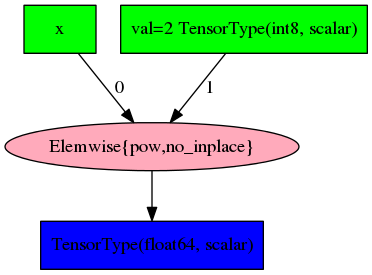
\includegraphics[width=3in]{Figures/yGraph.png}
	\caption[TheanoGraph]{Visualisation du graphe d'une fonction}
	\label{fig:Electron}
\end{figure}

	Les nœuds en verts sont les arguments de l'opérateur puissance (pow) qui est en bleu, et le résultat est dans le nœud en rose.
	Rappelons que lors de la phase d'apprentissage des réseaux de neurones (perceptrons multicouches et autres), il est nécessaire lors de la rétro-propagation du gradient de calculer des dérivés en fonctions de plusieurs paramètres. Theano nous facilite cela puis-que les dérivations s'effectuent simplement en appliquant la fonction \textit{grad}. 
Donc, la dérivée de la fonction \textbf{y} que nous avons défini, par rapport à \textbf{x} peut être calculer comme suit: \\

>> \textit{gy = T.grad(y, x)}\\

\textbf{gy} contient dorénavant la dérivée de \textbf{y} par rapport à \textit{x}, qui n'est rien d'autre que $2*x$ .\\

%>> \textit{theano.pp(gy)}\\
% '((fill((x ** TensorConstant{2}), TensorConstant{1.0}) * TensorConstant{2}) * (x ** (TensorConstant{2} - TensorConstant{1})))'\\
 
	En essayant d'afficher le graphe de \textbf{gy} nous obtenons la figure [Figure 4.2] ci-dessous:

\begin{figure}[H]
	\centering
		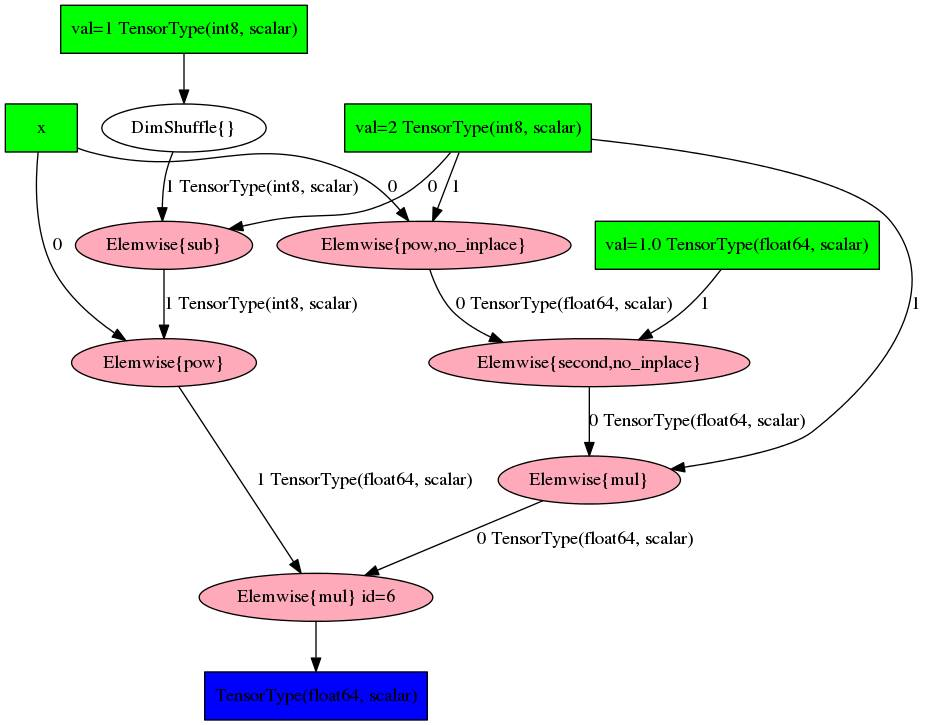
\includegraphics[width=5in]{Figures/beforeOptimization.png}
	\caption[TheanoGraph]{Visualisation du graphe de \textbf{gy} avant optimisation.}
	\label{fig:Electron}
\end{figure}

	Ce graphe n'est pas évident à comprendre alors qu'il s'agit seulement de la fonction $ gy = 2*x$. Compiler le graphe de \textbf{gy} à l'aide de la fonction "function" de Theano pour le rendre exécutable s'effectue comme suit:\\

>> \textit{f = theano.function([x], gy)}\\

	Cette opération optimise le calcul de \textbf{gy}, et le graphe de \textbf{f} devient comme le montre la figure ci-dessous:

\begin{figure}[H]
	\centering
		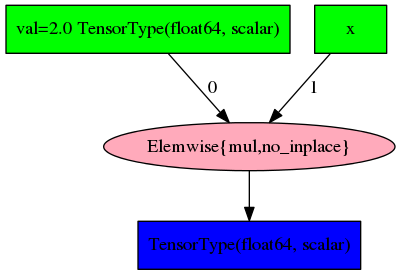
\includegraphics[width=3in]{Figures/afterOptimization.png}
	\caption[TheanoGraph]{Visualisation du graphe de \textbf{gy} après optimisation.}
	\label{fig:Electron}
\end{figure}

	Ceci montre à quel point Theano est puissant dans sa gestion des fonctions et de leurs dérivées, ainsi que leurs optimisation en quelques lignes de codes.
	
	Une notion très importante qui existe dans Theano est celle des \textit{variables symboliques}. Elle peuvent être considérées comme des tampons (buffers) qui contiennent des valeurs qui peuvent être partagées entre plusieurs fonctions de Theano.\\

	Un autre point fort de Theano est l'optimisation pour l'utilisation de matrices multi-dimensionnelles, mais aussi la facilité de compiler et exécuter les opérations sur des GPU au lieu des CPU.\\

	Theano fut suivi par d'autres frameworks qui ont repris les mêmes principes, les plus connus sont Tensorflow de Google, Blocks, Lasagne.

\subsection{Autres Frameworks}
	Theano n'étant pas évident à utiliser au début, pour remédié à ce problème, il existe d'autres frameworks qui ajoutent des couches d'abstraction à Theano pour faciliter son utilisation, comme Blocks, Lasagne et Keras.
	Le modèle VGG-CNN-S du réseau à convolution que nous avons utilisé dans notre algorithme est implémenté en Lasagne après avoir été converti de Caffe (Caffe étant un autre Framework en C++ développé par le laboratoire Berkeley Vision and Learning Center).\\

	Pour implémenté les autoencoders de nos approches, nous avons utilisé Blocks [Mer et al. 15], c'est un framework de theano qui facilite la définition de modèles et leur modifications. Il introduit des outils pour l'apprentissage, la visualisation et la sérialisation. Enfin, le framework Fuel [Mer et al. 15] permet de formater les données d'apprentissage d'une façon qui facilite leurs manipulation, surtout quand les tailles de ses dernières deviennent importantes.\\

	Dans notre cas, au lieu de le définir couche par couche, l'Autoencoder 4x1x4 est défini simplement par:\\

>> \textit{ae = MLP([Tanh(), Tanh()], [4096, 1000, 4096],
              weights\_init=IsotropicGaussian(0.01),
              biases\_init=Constant(0))\\
   }           

Puis, il est initialisé par:\\

>> ae.initialize()\\

	Ces deux frameworks sont développés aussi par le laboratoire MILA, ils forment une base solide pour le développement d’approches basées sur l'apprentissage profond.

\section{Interface de l'application}

	Après notre étude comparative dans le chapitre précédent entre les différentes approches que nous avons réalisé, nous avons décider d'implémenter dans l'interface graphique la meilleure approche (celle qui a donné les meilleures mesures de performance), qui est celle du Denoising Autoencoder 4x1x4.

	L'interface que nous avons développé pour l'implémentation de notre approche permet de sélectionner une base d'images qui servira de recueil pour les résultats des requêtes, comme le montre la figure [Figure 4.2].


\begin{figure}[H]
	\centering
		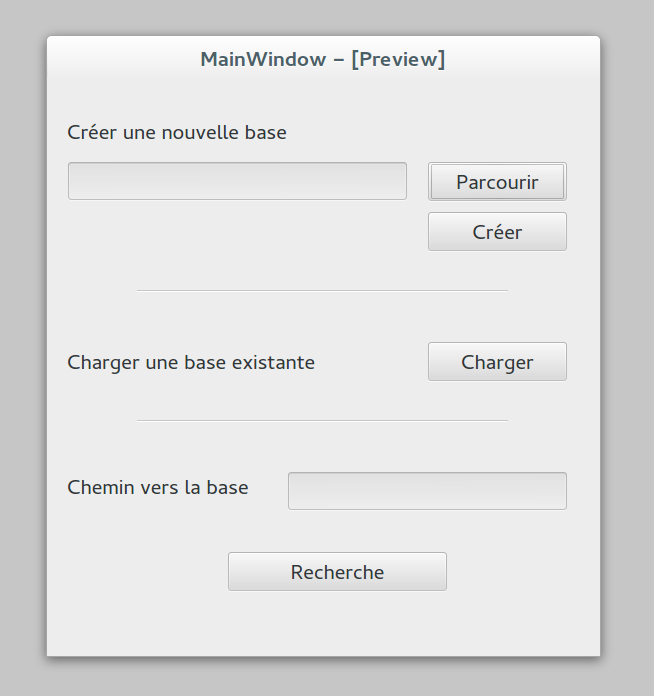
\includegraphics[width=3in]{Figures/mainMenu.png}
	\caption[Menu principal]{Menu principal}
	\label{fig:Electron}
\end{figure}

	Nous pouvons choisir de créer une nouvelle base, pour cela on doit indiquer le lien vers le dossier contenant la base d'images, puis appuyer sur le bouton \textit{Créer}. Le programme dans ce cas va créer la description de chaque image en la faisant passer par le réseau à convolution, ensuite extraire de la description sémantique de la couche 4096b et finalement créer la description compressée en utilisant le Denoising Autoencoder 4x1x4.
	C'est cette description qui sera enregistrée en tant que modèle pour la recherche d'images. On peut aussi charger une base déjà existante en appuyant sur le bouton \textit{Charger}.

	En cliquant sur le bouton "Recherche", une nouvelle fenêtre s'ouvre qui permet de sélectionner une image qui fera office de requête [Figure 4.3]. Une fois l'image sélectionnée, le programme va créer sa représentation sémantique compressée. Le bouton "Chercher" lance la recherche et affiche les cinq images jugées les plus ressemblantes (top-5).

\begin{figure}[H]
	\centering
		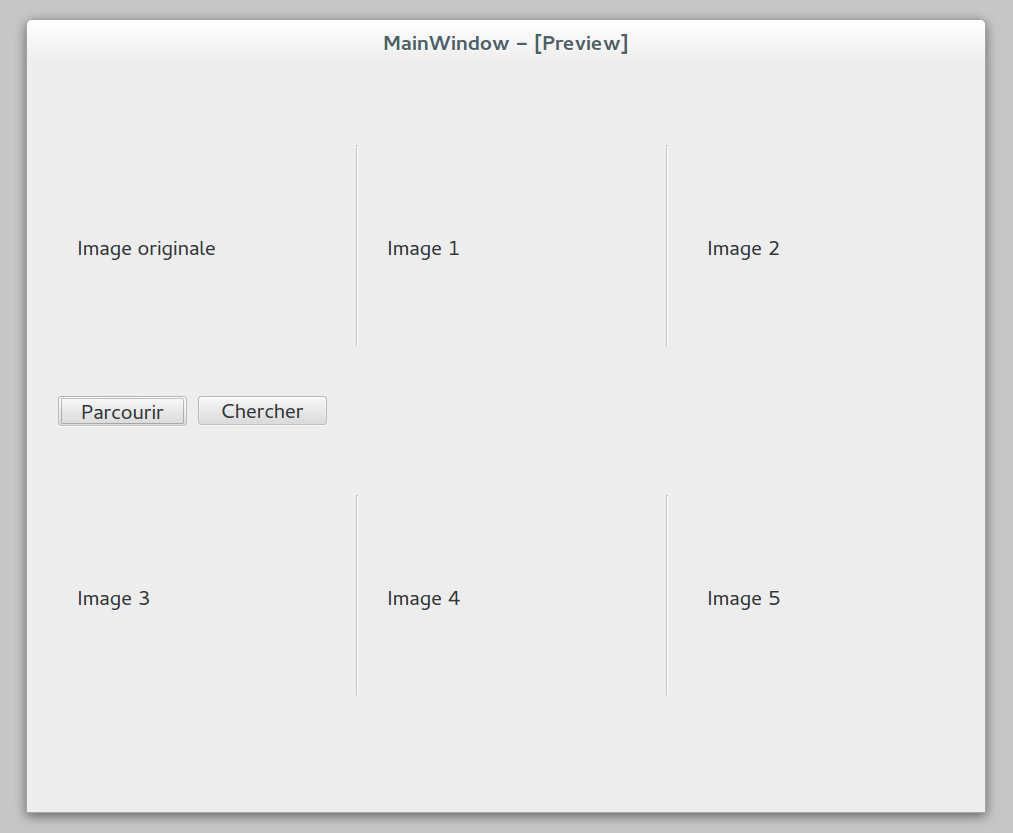
\includegraphics[width=5in]{Figures/search.png}
	\caption[]{Interface de recherche d'images.}
	\label{fig:Electron}
\end{figure}

\section{Tests}

Nous avons pris quelques images pour effectuer des testes sur les bases de donne WANG et AUTRE.

\section{Conclusion}

Nous concluons ce chapitre.
